\chapter{Implementation}
This section discusses the implementation of the music social network it is split into the multiple stories which have previously been listed.

\section{The Registration System}
\subsection{Back End}
Work began on the registration system by creating the appropriate tables on the back end. These tables were user\_types, users, genres and user\_genres. The user types table contained the three different types of account which a user could have: Music Lover, Artist and Venue Owner. The user type was done as a separate table to the users table itself for extensibility purposes as if additional user types needed to be added they could just simply be added to the table. The users table just contained all of the users' details including name, display name, email, password (discussed in more depth during the security section) and a url link to their picture. The genres table was simply a table which contained different genres of music and an appropriate id for each genre and as genres to users is a many to many relationship a users\_genres table was stored a user\_id and a genre\_id.

After the tables had been created the php files (hosted at seananderson.co.uk/api) were created. These php files essentially formed the RESTful API which would allow for the front end to connect to the database for the system. The first file which was created was register.php this file takes variables which the user passes in (through POST data) and adds them to the database via my sql commands which are ran from within the php. Some validation was done in the php file to check that things such as the email given are valid emails however I wanted to do most of the validation actually on the front end as this would allow for error messages to get out to the user quicker. 

As at this stage in time there was no front end it was not possible to test that sending post data from an app would work. So, a piece of software called postman (which is a Google Chrome extension) was used as this software allows for post data to be pushed to a website as illustrated in figure X. As well as relying on the PHP file telling me 'A new user was added successfully' which is the message what is printed when the sql commands all run correctly the database was also checked to ensure that the new user had been added correctly as shown in figure X.

Having completed this stage I did notice a significant weakness in using hybrid technology, the act
\begin{figure}[H]
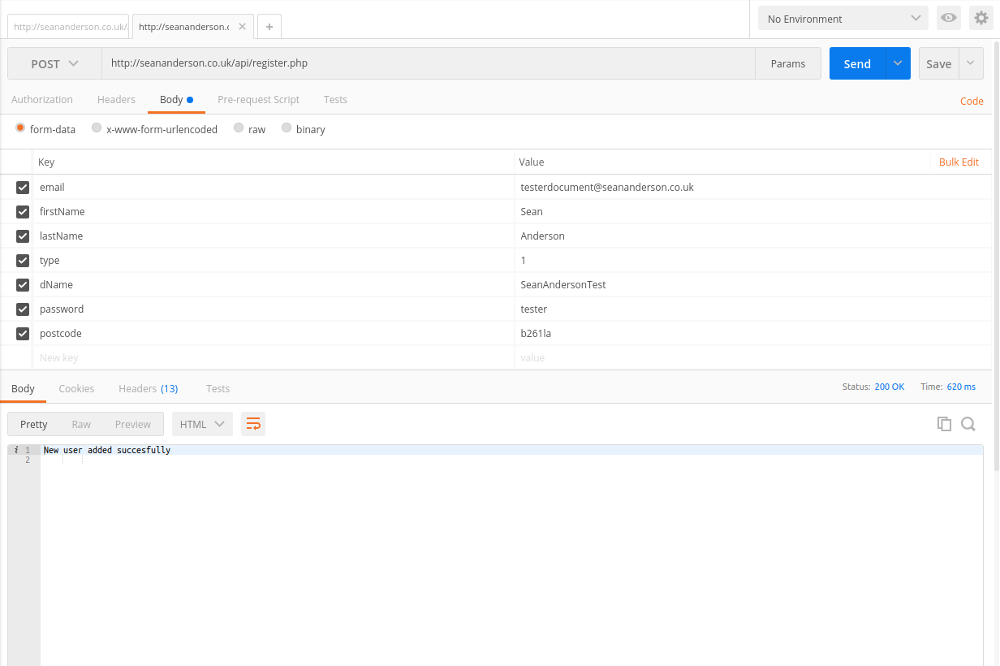
\includegraphics[scale=0.45]{images/postman}
\caption{Postman testing register.php}

\includegraphics[scale=0.45]{images/db1}
\caption{User added to the database}
\end{figure}

For setting up registering different users' genres the system was implemented in the exact same way as the registration system only that there was far fewer variables. The login API simply checks that the user provides an email and password and that they match and if they do match returns the user details and if they don't match returns a message saying that the password is not correct.

\subsubsection{Security within the Registration System}
It is important that users are not allowed to enter dangerous characters into the database, as a result of this all strings which will be imputed for the user (for all backend files for the music social media) are escaped using the mysqli\_escape function which is a default php function which ensures that any characters which could potentially do damage to the database are escaped and therefore not ran in the mysqli statements.

As the registration and login system used a password it was important to ensure that if somebody was to get access to the database that they wouldn't get access to the password. There are multiple different methods of encryption which could have been used for this. PHP has its own built in function called password\_hash which takes in two parameters the password itself as a string and the encryption type. For this project password\_default which is a predefined php hashing method was used. Password default was used as it was a simplistic and relatively secure way of turning a password into a hash. The password\_verify function in PHP is used to check that a plain text password matches the hashed password.
 
\subsection{Front End}
After the back end for the registration of the app was created development then started on the front end of the app. The default ionic menu bar template was used as this would allow for a menu bar to appear on multiple pages (like in my design) easily.

The views for both the login and registration system were created using html (as are all views in ionic) and the controllers for those views were created in AngularJS and were simply js files. Both the register and login view files contained a form which gathered appropriate information from the user and then passed that information onto the controllers when submitted. The controllers then passed that information onto the API's by using \$http.post which is an AngularJS method used for calling post api's.
\begin{verbatim}
$http.post(api, data).then(function(res){
  apiReturns = JSON.stringify(res);
  if (apiReturns.includes('New user added succesfully')>=0) {
    localStorage.setItem('email', $scope.register.email);
    localStorage.setItem('dName', $scope.register.dName);
    if ($scope.registerGenre!=undefined) {
      $scope.registerGenre();
    }
    $state.go('app.profile');
    popUp('Welcome', 'Welcome to Dynamic please fill in your profile page and then follow some users');
  }
})

\end{verbatim}

In passing the information from the controller to the API I encountered a problem. AngularJS sends post data in a different way to most other languages. As a result of this the following lines of code had to be added to the PHP files. (This code was taken from \url{http://corpus.hubwiz.com/2/angularjs/15485354.html})
\begin{verbatim}

if ($_SERVER['REQUEST_METHOD'] == 'POST' && empty($_POST)) {
    $_POST = json_decode(file_get_contents('php://input'), true);
}

\end{verbatim}

Figure 3.3 shows what the front end for the login and registration screens look like on the front end on the system (from the perspective of a One Plus Two device.)

\begin{figure}[H]
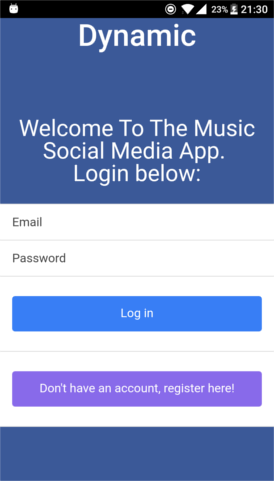
\includegraphics[scale=0.5]{images/sc1}
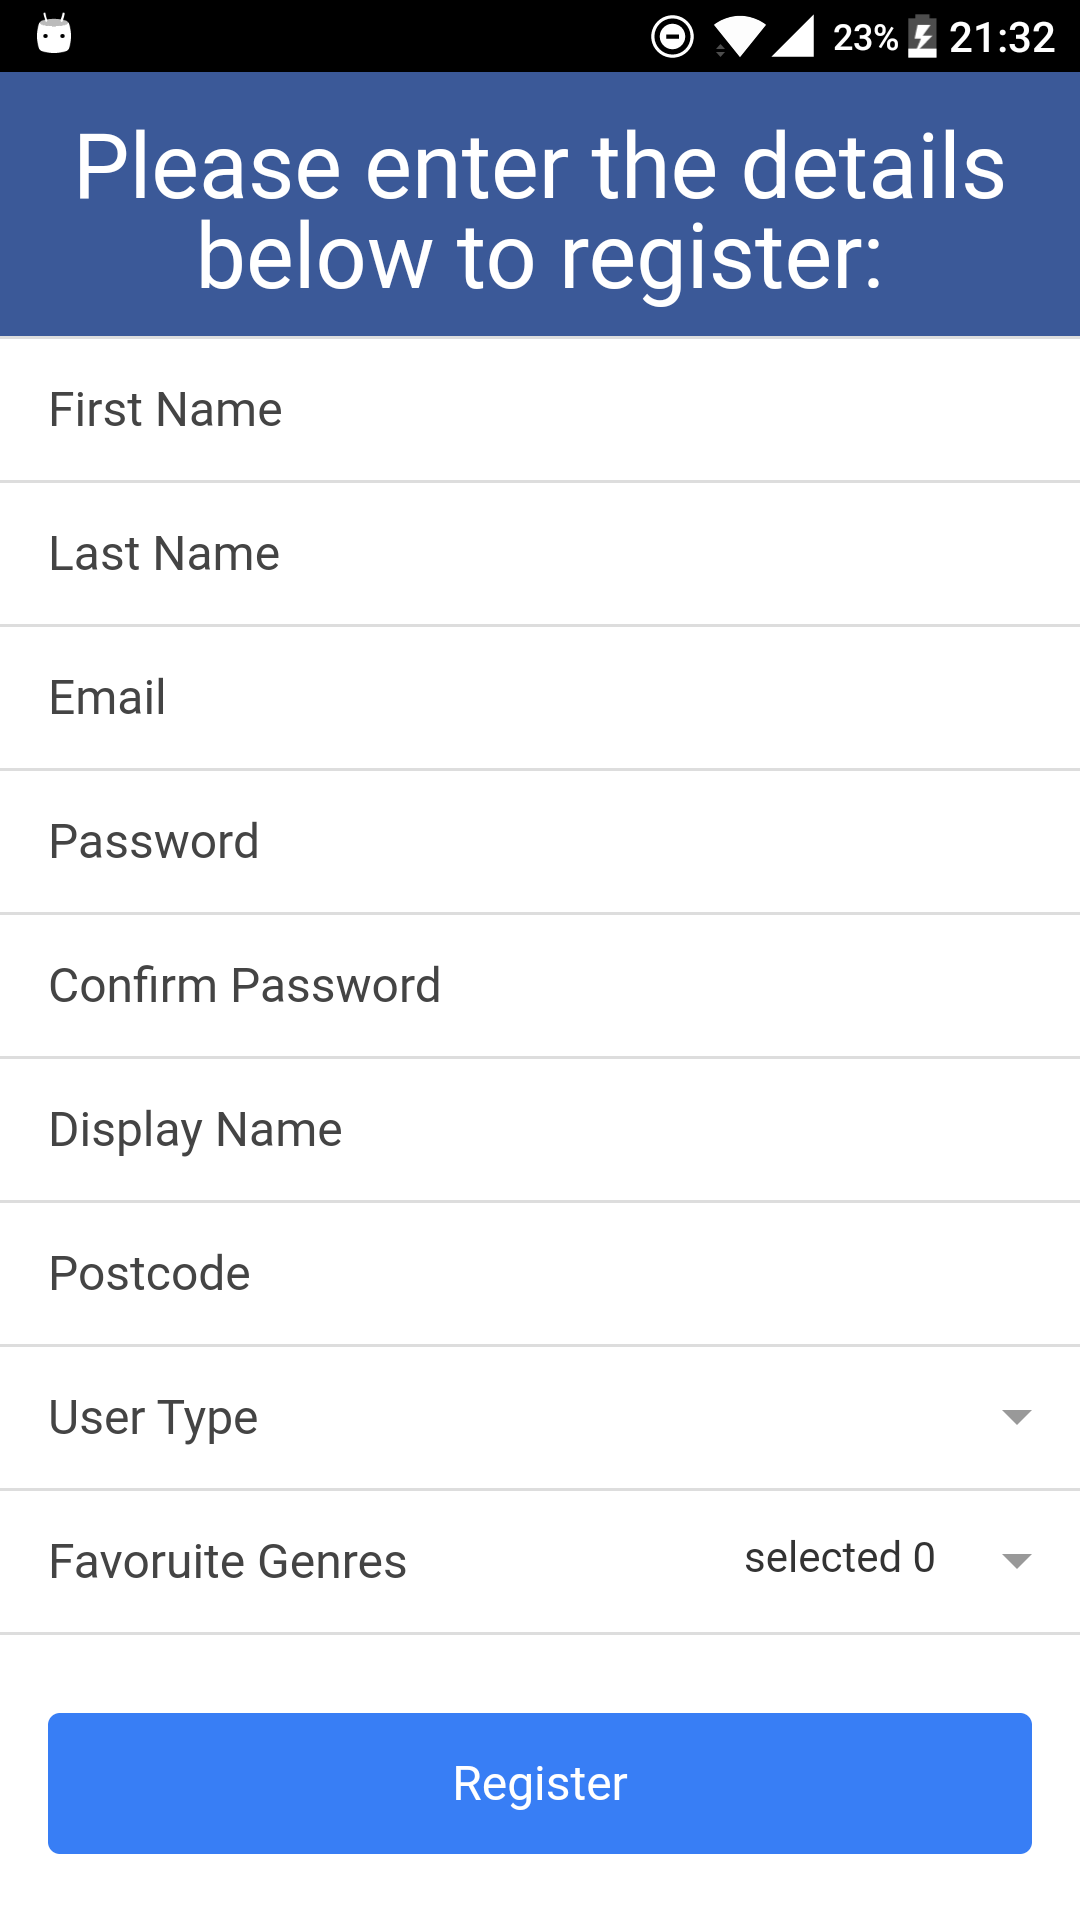
\includegraphics[scale=0.5]{images/sc2}
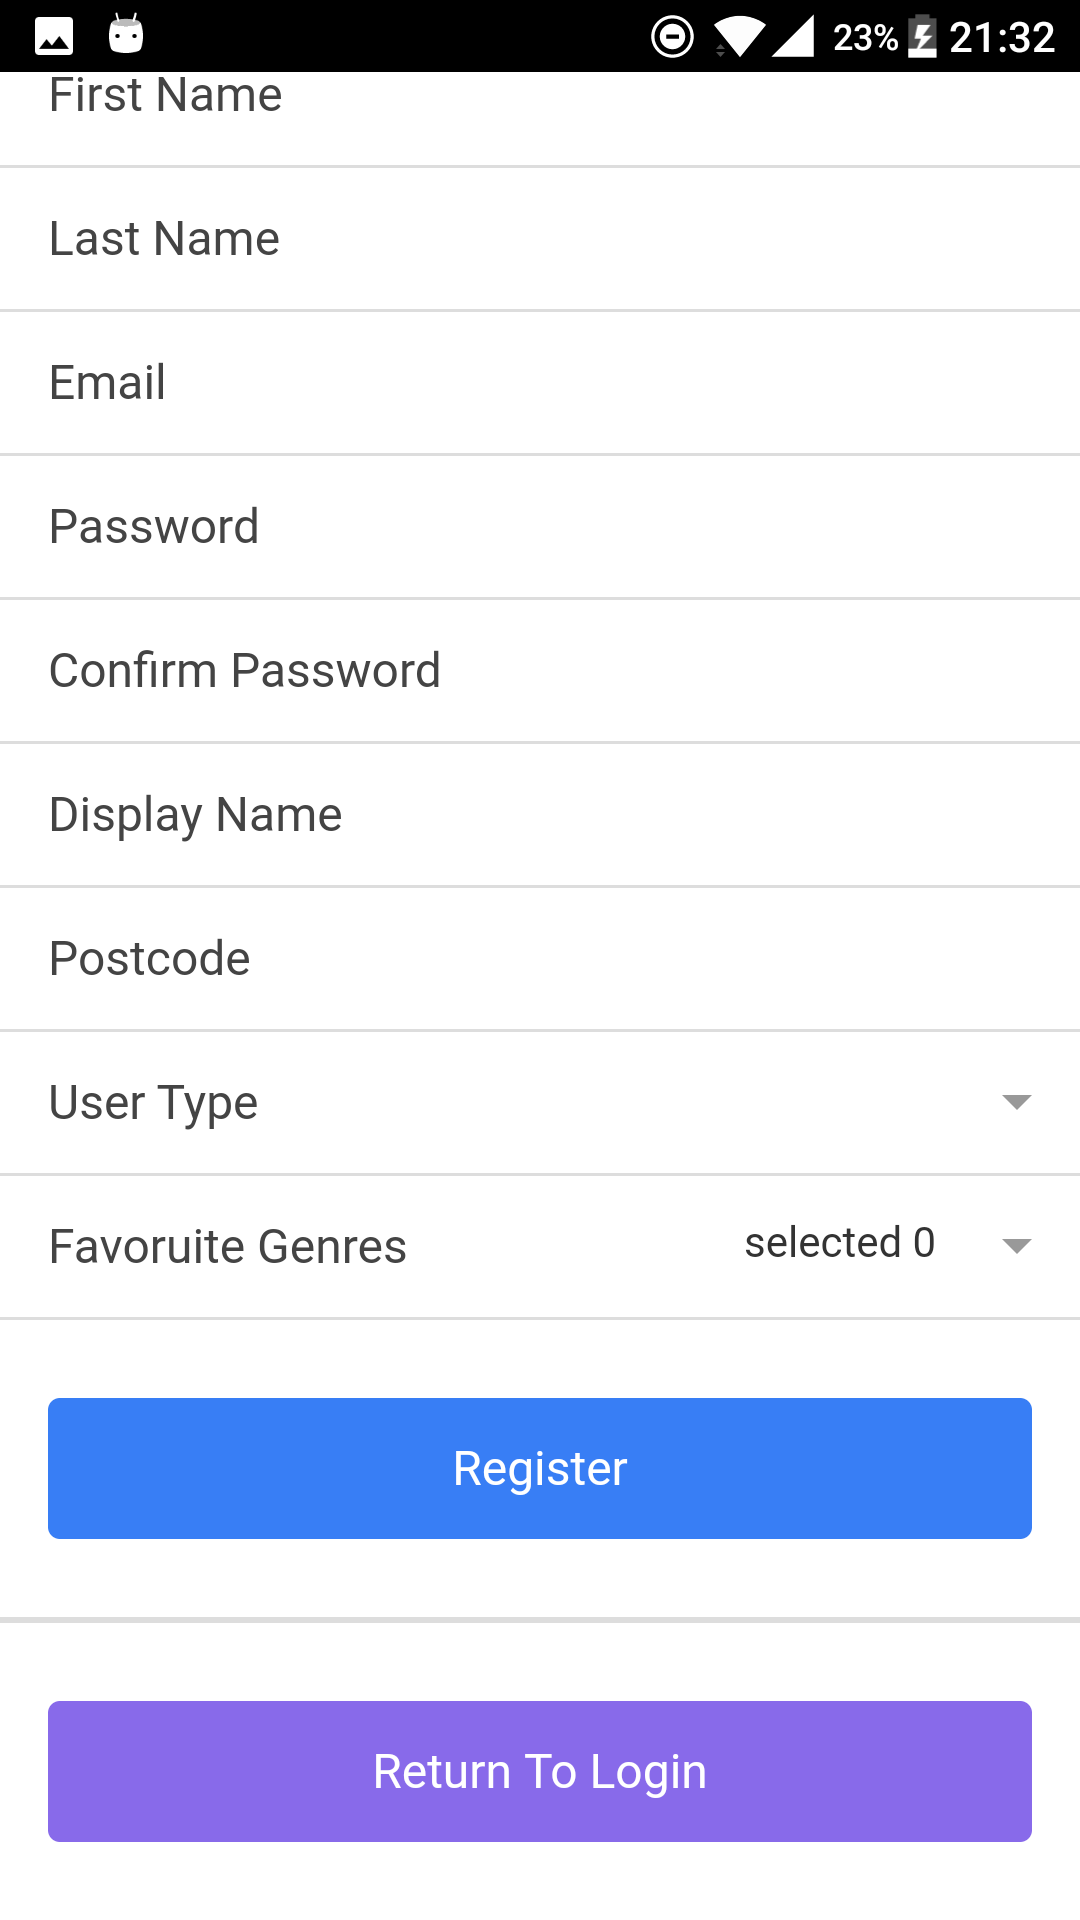
\includegraphics[scale=0.5]{images/sc3}
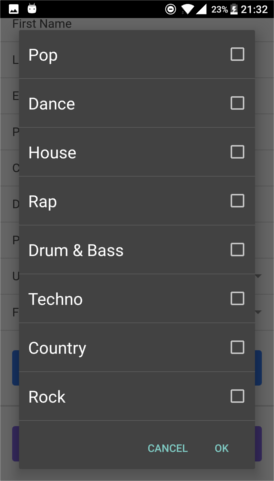
\includegraphics[scale=0.5]{images/sc4}
\caption{Screenshots of registration system.}
\end{figure}

\subsection{Validation}
Having successfully got the front end interacting with the back end it was important to ensure that all of the data being sent over was valid. I decided first of all to validate the data on the front end so I ensured that the user had filled in all of the appropriate boxes and used a regex to ensure that the email address they entered was correct.

It was then necessary to create some more API files as each user had to have a unique email and display name files called checkemail.php and displayname.php were created these files run SQL queries to ensure that the email address and display name which the user entered are unique.

Figure 3.4 displays an example of what happens when a user tries to register an account with an email address which has already been used and when a password is not long enough.

\begin{figure}[H]
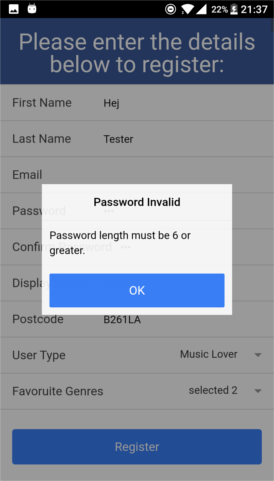
\includegraphics[scale=0.5]{images/sc5}
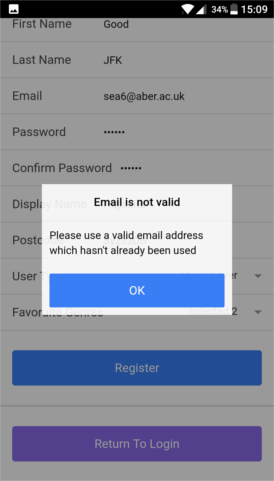
\includegraphics[scale=0.5]{images/sc6}
\caption{Validation Screenshots}
\end{figure}

\section{Users Profile}
Having created the registration and login system the next story to tackle was allowing the user to add a bio and to upload a picture. This picture would act as the users profile picture. Having previously completed the registration system allowing the user to add a bio was rather straightforward. It was just simply a matter of creating a front end which passes a variable to a  php file (called update bio.php), the php files then takes the post variable and turns it into a php variable. Finally the php file runs a sql command which updates the users table to have the correct information for the bio.

\subsection{Camera and FileTransfer Plugins}
The task of allowing a user to upload a profile picture can be broken down into two seperate tasks. The task of actually allowing the user to take the photo or pick a photo from their devices library, and the ask of transferring that photo to the backend. 

Installing the cordova camera plugin \cite{cc} was necessary to allow the user to take a photo or select a photo from their devices library. The actual installation of the plugin was simple, following the documentation for the plguin was straightforward and the app was programmed so that if the user clicked a button saying upload a picture or choose a picture from my gallery then the Cordova Camera plugin was called with the correct options configured.

Figure 3.4 highlights the two different buttons and what happens when they are clicked.

\begin{figure}[H]

\includegraphics[scale=0.5]{images/cs}
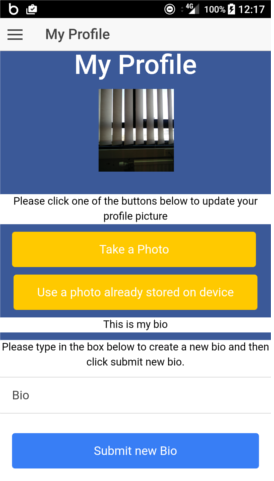
\includegraphics[scale=0.5]{images/sc7}
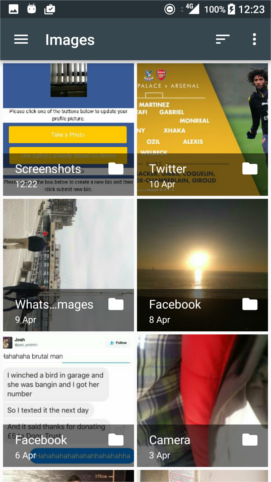
\includegraphics[scale=0.5]{images/sc9}
\caption{Screen shot of camera functionality.}
\end{figure}

After the user confirms (by pressing the tick) that they want to use the photo as their profile picture the photo is then uploaded to the server. The first step in getting the  the photo to upload was to create a API file, this file was entitled imageupload.php and is hosted at seananderson.co.uk/api/imageupload.php. This file contains some fairly trivial code which just gets the data of the image which has been uploaded and places it in an appropriate folder (seananderson.co.uk/api/uploads). Afer creating the php file the next step was to pass the photo from the device to the server. This was done by using the Cordova File Transfer plugin \cite{ft}. This plugin simply takes a file (which in this case was the image) and uploads the file to the specified URL
After implementing the camera plugin one clear disadvantage of hybrid apps became apparent. The time taken for the device to take a picture and then process that picture was significantly longer than it takes when using a native app. This will be discussed in more depth during the testing section of this report. 

\subsubsection{Caching Issue}
At this stage of the development of the app it became apparent that there was an issue with caching. The issue was noticed as when the picture loaded on the users profile page after the user uploaded a new picture the picture would not be updated. 

A variety of different ways was used to try and tackle the issue. Ionic allows for the apps cache to be cleared using \$ionicHistory.clearCache(); however this unfortunately didn't resolve this issue. As clearing the apps cache wasn't getting rid of the issue it was clear that the problem lied within the browser (which is how the app is ran.)

It turned out that the Chrome browser was caching the results of the API which displayed the picture, as the same API was being called on the page refresh, which was ran once the photo was uploaded. Despite not being the most elegant solution a random number was added to the end of the pictures url.

\begin{verbatim}
$http.post(api, data, { cache: false }).then(function(res){
  //Below line is a hack, justified in report.
  var image = (res['data']['picture']) + '?random=' + Math.random();
  var photoDiv = angular.element(document.querySelector('#profile-photo'));
  photoDiv.html('<div id ="profile-photo"><img  height="60 px" 
  width="60 px" src="' + image + '"</img></div>');
})

\end{verbatim}

This meant that the browser would load the new image uploaded into the app as it would have a different url from the old image. The caching issue is clearly a negative to hybrid app development, if the app was developed in a native manner then it would allow for 

\subsubsection{Problem with Different Devices}
The image camera plugin worked fine on a One Plus Two mobile phone, however when the functionality was tested using a Samsung Galaxy A there was a problem, the orientation of the image was wrong. The Samsung Tablet would take the photo fine but when it actually came to uploading it, it would rotate the image. 

One of the options when using the camera plugin is photo orientation. 
\begin{verbatim}
var options = {
  quality:80,
  targetWidth:500,
  targetHeight:750,
  sourceType : Camera.PictureSourceType.CAMERA,
  encodingType: Camera.EncodingType.PNG,
  correctOrientation: true
};
\end{verbatim}
Unfortunately enabling that to be true still didn't solve the problem. Despite there not being any official sources suggesting why the correct orientation doesn't always work the feeling within the Ionic Community is that Samsung devices actually ignore the  
\section{Styling}
As ionic uses HTML for its views the styling is done in CSS, SASS can be used as an alternative to CSS if the developer wants. The majority of the app was styled whilst working on each story however it was important to spend some time to ensure that the styling of the app was consistent.

This did actually bring up some issues with hybird app development. Whilst a key feature of hybrid app development is the ability to deploy an app to multiple different code bases; iOS and Android interpret CSS differently. Therefore time had to be spent tweaking the CSS of the iOS version. (Add this if possible Figure X shows a particular part of the app running on iOS and Android however it is clearly inconsistent.)

\section{Technical Challenges}
There was multiple technical challenges which were faced when developing the app. The first of which was actually learning AngularJS, this was simply a case of trying different things until they worked and looking at multiple different sources online.

The caching issue was a rather interesting technical challenge, despite it not taking a long time to resolve it clearly highlighted an issue with hybrid mobile apps. The photo orientation with the multiple different devices was also an issue as it meant that more lines of php had to be added to the API to ensure that the photo was uploaded in right orientation, therefore a developer would have to spend more time working on the photo upload using hybrid technologies than if they were to use the native app development.            
\section{Actual Implementation vs Plan}
